\documentclass[11pt,a4paper]{article}
\usepackage[utf8]{inputenc}
\usepackage[T1]{fontenc}
\usepackage[brazil]{babel}
\usepackage{lmodern}
\usepackage{amsmath,amssymb}
\usepackage{booktabs,array,longtable}
\usepackage{graphicx}
\usepackage{xcolor}
\usepackage{listings}
\usepackage[margin=2.3cm]{geometry}
\usepackage{caption,subcaption}
\usepackage{float}
\usepackage{tikz}
\usepackage{pgfplots,pgfplotstable}
\usepackage[hidelinks]{hyperref}
\usetikzlibrary{positioning,arrows.meta,calc,fit,backgrounds,shapes.geometric}
\pgfplotsset{compat=1.18}
\usepgfplotslibrary{groupplots}
\setlength{\emergencystretch}{3em}

% painel do ciclo de marcha: #1 variavel, #2 lado da simulacao (R/L), #3 cor
\newcommand{\cyclepanel}[3]{%
  \addplot[fill=black!15, draw=none, forget plot] table[x=bx, y=hS_#1] {\faixas};
  \addplot[fill=#3, fill opacity=0.25, draw=none, forget plot] table[x=bx, y=s#2_#1] {\faixas};
  \addplot[black!70, thick, forget plot] table[x=pct, y=hS_#1_m] {\ciclo};
  \addplot[black!70, dashed, forget plot] table[x=pct, y=hC_#1_m] {\ciclo};
  \addplot[#3, very thick, forget plot] table[x=pct, y=s#2_#1_m] {\ciclo};
}
% legenda comum das figuras de ciclo
\newcommand{\cyclelegend}{%
\begin{tikzpicture}[font=\footnotesize]
  \fill[black!15] (0,0) rectangle (0.6,0.25); \draw[black!70, thick] (0,0.125) -- (0.6,0.125);
  \node[right] at (0.65,0.125) {saudável lento, média $\pm$1 DP};
  \draw[black!70, dashed] (4.9,0.125) -- (5.5,0.125); \node[right] at (5.55,0.125) {saudável confortável};
  \fill[cOrange, opacity=0.25] (8.9,0) rectangle (9.5,0.25); \draw[cOrange, very thick] (8.9,0.125) -- (9.5,0.125);
  \node[right] at (9.55,0.125) {simulação, prótese};
  \fill[cBlue, opacity=0.25] (12.5,0) rectangle (13.1,0.25); \draw[cBlue, very thick] (12.5,0.125) -- (13.1,0.125);
  \node[right] at (13.15,0.125) {simulação, intacta};
\end{tikzpicture}}

\usepackage{url}
\DeclareUrlCommand\code{\urlstyle{tt}}
\makeatletter\g@addto@macro\UrlBreaks{\do\_\do\-}\makeatother
\definecolor{cOrange}{RGB}{217,84,26}
\definecolor{cBlue}{RGB}{0,114,189}
\definecolor{cGreen}{RGB}{60,140,60}
\definecolor{cGray}{RGB}{110,110,110}
\definecolor{codebg}{RGB}{248,248,248}

\lstdefinelanguage{Matlab}{
  morekeywords={function,end,if,else,elseif,for,while,switch,case,otherwise,try,catch,return,break,
    classdef,properties,methods,import,parfor,persistent,global},
  sensitive=true, morecomment=[l]\%, morestring=[m]', morestring=[b]"}
\lstset{
  language=Matlab, basicstyle=\ttfamily\scriptsize, keywordstyle=\color{cBlue}\bfseries,
  commentstyle=\color{cGreen}\itshape, stringstyle=\color{cOrange}, backgroundcolor=\color{codebg},
  numbers=left, numberstyle=\tiny\color{cGray}, frame=single, rulecolor=\color{black!20},
  breaklines=true, columns=fullflexible, keepspaces=true, showstringspaces=false, tabsize=4,
  extendedchars=true, literate={°}{{\textdegree}}1 {—}{{---}}1}

\title{\textbf{Simulação de marcha de amputado transfemoral com prótese passiva:\\
dinâmica direta OpenSim integrada no MATLAB e controle muscular por aprendizado por reforço}\\[4pt]
\large Relatório técnico do projeto \code{RL_OSim}}
\author{}
\date{5 de novembro de 2026}

\begin{document}
\maketitle

\begin{abstract}
Este relatório documenta o código desenvolvido para simular, por dinâmica direta, a marcha de um
amputado transfemoral direito com o modelo OpenSim \code{OS4_gait14dof15musc_2Act_RTFP_DynAct.osim}.
Joelho e tornozelo protéticos são \emph{passivos} (mola e amortecedor), e os 15 músculos do modelo são
controlados por um agente \emph{Soft Actor-Critic} (SAC) que aprende correções sobre um controlador-base
de rastreamento. Toda a integração das equações diferenciais é feita no MATLAB (\code{ode23}); o OpenSim
apenas avalia $\dot{\mathbf y}=f(t,\mathbf y,\mathbf e)$. A recompensa segue o estilo DeepMimic: imita a
cinemática de marcha saudável, busca 1{,}2~m/s e penaliza esforço e variações bruscas de excitação.
Depois de 150 blocos de 40 episódios, o melhor agente anda 20~s sem cair a partir de qualquer fase inicial
testada, a 0{,}94~m/s e com assimetria de apoio de 11\,\%. Ele atende 3 dos 5 critérios de plausibilidade
fisiológica adotados. O relatório descreve a arquitetura, a função de recompensa, as redes neurais, o
procedimento de treino, os resultados e cada arquivo do código.
\end{abstract}

\tableofcontents
\newpage

%=====================================================================
\section{Objetivo e requisitos}
%=====================================================================
O objetivo é emular, no modelo de um amputado transfemoral, uma marcha com prótese o mais próxima possível
da marcha humana saudável, controlando os músculos do modelo por aprendizado por reforço até que o
movimento seja suave o bastante para parecer fisiologicamente possível. Os requisitos fixados ao longo do
projeto foram:
\begin{enumerate}
  \item \textbf{Modelo:} \code{OS4_gait14dof15musc_2Act_RTFP_DynAct.osim} (amputação transfemoral direita).
  \item \textbf{Músculos controlados} (15): \code{abd_r}, \code{add_r}, \code{glut_max_r}, \code{iliopsoas_r}
        (coto) e \code{abd_l}, \code{add_l}, \code{hamstrings_l}, \code{bifemsh_l}, \code{glut_max_l},
        \code{iliopsoas_l}, \code{rect_fem_l}, \code{vasti_l}, \code{gastroc_l}, \code{soleus_l},
        \code{tib_ant_l} (perna intacta).
  \item \textbf{Integração da ODE no MATLAB}, não no OpenSim (o \code{Manager} do OpenSim não é usado).
  \item \textbf{Prótese passiva:} joelho e tornozelo sem nenhum controle ativo, como em próteses passivas reais.
\end{enumerate}

%=====================================================================
\section{Arquitetura geral}
%=====================================================================
A Figura~\ref{fig:loop} mostra o laço de controle. A cada passo de controle de 10~ms, o agente lê uma
observação de 63 elementos e devolve 15 resíduos de excitação. Esses resíduos passam por um filtro
passa-baixa e são somados às excitações do controlador-base. As excitações resultantes ficam constantes
durante o passo (\emph{zero-order hold}) enquanto o \code{ode23} do MATLAB integra o modelo OpenSim.

\begin{figure}[H]
\centering
\begin{tikzpicture}[
  font=\small, >={Stealth[length=2.2mm]},
  blk/.style={draw, rounded corners=2pt, align=center, minimum height=1.0cm, inner sep=4pt, fill=white},
  sumn/.style={draw, circle, inner sep=1.2pt, fill=white},
  lbl/.style={font=\scriptsize, align=center, inner sep=1pt}]
  \node[blk, fill=cBlue!12, minimum width=2.6cm] (actor) at (0,0) {Ator SAC\\ $\pi_\phi(\mathbf a\,|\,\mathbf o)$};
  \node[blk, minimum width=3.4cm] (filt) at (4.9,0) {Filtro passa-baixa\\ $\mathbf u_k=0{,}5\,\mathbf u_{k-1}+0{,}5\,\mathbf a_k$};
  \node[sumn] (sum) at (7.9,0) {$+$};
  \node[blk, minimum width=2.1cm] (sat) at (10.1,0) {Saturação\\ $[0{,}01,\;1]$};
  \node[blk, fill=cGreen!10, text width=4.6cm] (base) at (5.9,-2.4)
       {Controlador-base: PD articular + equilíbrio do tronco (SIMBICON) $\to$ torques $\to$ excitações (\code{lsqnonneg})};
  \node[blk, fill=cOrange!10, text width=4.1cm] (plant) at (11.9,-2.6)
       {\textbf{Modelo OpenSim}\\ 15 músculos Thelen2003\\ contato Hunt--Crossley\\ prótese passiva (mola + amortecedor)\\[2pt]
        $\dot{\mathbf y}=f(t,\mathbf y,\mathbf e)$\\ via \code{realizeAcceleration}};
  \node[blk, fill=cOrange!20, text width=4.1cm] (ode) at (11.9,-5.6)
       {\textbf{MATLAB} \code{ode23}\\ integra $[t,\,t+10\,\mathrm{ms}]$ com $\mathbf e$ constante};
  \node[blk, minimum width=2.6cm] (obs) at (4.6,-5.6) {Observação\\ $\mathbf o\in\mathbb R^{63}$};
  \node[blk, fill=cBlue!5, minimum width=2.6cm] (rew) at (4.6,-7.8) {Recompensa $r_k$\\ (imitação, velocidade,\\ esforço, suavidade)};
  \node[blk, fill=cBlue!12, minimum width=2.6cm] (learn) at (0,-7.8) {Aprendiz SAC\\ (2 críticos $Q$,\\ buffer $10^6$)};
  % setas
  \draw[->] (actor) -- node[lbl, above=3pt]{$\mathbf a\in[-1,1]^{15}$} (filt);
  \draw[->] (filt) -- node[lbl, above=3pt]{$0{,}25\,\mathbf u$} (sum);
  \draw[->] (base.north -| sum) -- node[lbl, right=2pt]{$\mathbf e_{\mathrm{base}}$} (sum);
  \draw[->] (sum) -- (sat);
  \draw[->] (sat.south) -- node[lbl, left=2pt]{$\mathbf e\in\mathbb R^{15}$\\ excitações} (sat.south |- plant.north);
  \draw[->] (plant) -- node[lbl, right=2pt]{$\dot{\mathbf y}$} (ode);
  \draw[->] (ode.west) -- node[lbl, above=3pt]{estado $\mathbf y\in\mathbb R^{66}$} node[lbl, below=3pt]{$[\mathbf q;\dot{\mathbf q};\mathbf z]$} (obs.east);
  \draw[->] (obs.north) -- node[lbl, left=2pt]{$\mathbf q,\dot{\mathbf q}$,\\ fase, GRF} (obs.north |- base.south);
  \draw[->] (obs.west) -| ($(actor.south)+(0.6,0)$);
  \draw[->] (ode.south) |- (rew.east);
  \draw[->] (rew) -- node[lbl, above=3pt]{$(\mathbf o,\mathbf a,r,\mathbf o')$} (learn);
  \draw[->, dashed] ($(learn.north)+(-0.6,0)$) -- node[lbl, left=2pt, pos=0.5]{atualiza\\ $\phi$} ($(actor.south)+(-0.6,0)$);
\end{tikzpicture}
\caption{Laço de controle. O OpenSim só avalia as derivadas; a integração é feita pelo \protect\code{ode23} do
MATLAB. O agente produz resíduos sobre o controlador-base, e a prótese não recebe nenhum comando.}
\label{fig:loop}
\end{figure}

\begin{table}[H]
\centering\small
\caption{Divisão de responsabilidades.}
\begin{tabular}{@{}p{4.4cm}p{10.8cm}@{}}
\toprule
Parte & Onde \\ \midrule
Equações do modelo, $\dot{\mathbf y}=f(t,\mathbf y,\mathbf e)$ & OpenSim 4.4 (API Java): \code{setY} $\to$ \code{realizeAcceleration} $\to$ \code{getYDot} \\
Integração da ODE & MATLAB, \code{ode23} (RelTol $10^{-3}$, AbsTol $10^{-4}$) \\
Controle (constante por 10~ms) & MATLAB: controlador-base + resíduo do agente \\
Aprendizado por reforço & MATLAB Reinforcement Learning Toolbox, agente SAC, 4 workers em paralelo \\
\bottomrule
\end{tabular}
\end{table}

%=====================================================================
\section{Modelo musculoesquelético e prótese passiva}
%=====================================================================
O modelo tem pelve, tronco, perna esquerda intacta e o lado direito amputado: coto femoral
(\code{transfemur}), encaixe osseointegrado (\code{osseo_pylon}), pilão tibial (\code{tibia_pylon}) e pé
protético (\code{foot_r}). Os 15 músculos são do tipo Thelen2003. O contato com o solo usa esferas
Hunt--Crossley no calcanhar e na ponta de cada pé (\code{foot_r}, \code{foot_l}).

\paragraph{Estágio planar.} Para o primeiro estágio, a marcha é restrita ao plano sagital, com abdução e
adução do quadril livres. Ficam travadas as coordenadas \code{pelvis_list}, \code{pelvis_rotation},
\code{pelvis_tz} e \code{hip_rotation_r} (\code{gaitConfig('planar', true)}, o padrão).

\paragraph{Prótese passiva.} Os atuadores ativos do modelo, \code{knee_actuator} e \code{ankle_actuator},
são desligados (\code{set_appliesForce(false)}). Em cada junta protética entra um
\code{SpringGeneralizedForce} que aplica
\begin{equation}
\tau_{\mathrm{prot}} = -k\,(q-q_0) - b\,\dot q ,
\end{equation}
com os valores da Tabela~\ref{tab:prot}. Os batentes \code{KneeLimit_r} e \code{AnkleLimit_r} do modelo
continuam ativos. Assim, joelho e tornozelo direitos só se movem pela dinâmica do corpo e pelas forças dos
músculos do coto sobre o fêmur residual, como numa prótese passiva real.

\begin{table}[H]
\centering\small
\caption{Parâmetros da prótese passiva (\protect\code{c.prosthesis} em \protect\code{gaitConfig.m}).}
\label{tab:prot}
\begin{tabular}{@{}p{3.6cm}cccp{6.2cm}@{}}
\toprule
Junta & $k$ (N\,m/rad) & $b$ (N\,m\,s/rad) & $q_0$ & Interpretação \\ \midrule
Joelho (\code{knee_angle_r}) & 5 & 3 & 0 & joelho mecânico com atrito hidráulico simples e leve mola de extensão \\
Tornozelo (\code{ankle_angle_r}) & 350 & 2 & 0 & pé de armazenamento de energia (ESAR), $\approx$6~N\,m/grau \\
\bottomrule
\end{tabular}
\end{table}

\paragraph{Assistência na pelve.} O código cria também atuadores de coordenada na pelve (\code{assist_*}),
uma ``mão de Deus'' para currículo. Na execução final eles ficam desligados (\code{assistStart = 0}),
e toda avaliação é feita sem assistência.

%=====================================================================
\section{Dinâmica direta integrada no MATLAB}
%=====================================================================
O estado do Simbody tem 66 variáveis:
\begin{equation}
\mathbf y = \big[\,\mathbf q\in\mathbb R^{17};\ \dot{\mathbf q}\in\mathbb R^{17};\ \mathbf z\in\mathbb R^{32}\,\big],
\end{equation}
em que $\mathbf z$ reúne 15 ativações musculares, 15 comprimentos de fibra e 2 ativações dos atuadores
protéticos desligados, que ficam inertes. A função \code{dynamics} do ambiente é o lado direito da ODE:
\begin{lstlisting}[firstnumber=238]
function yd = dynamics(this, s, t, y)
    s.setTime(t);
    s.setY(org.opensim.modeling.Vector.createFromMat(y));
    this.model.realizeAcceleration(s);
    yd = s.getYDot().getAsMat();
end
\end{lstlisting}
Em cada passo de controle $k$, as excitações $\mathbf e_k$ são gravadas em funções \code{Constant} de um
\code{PrescribedController}, e o MATLAB integra o intervalo:
\begin{equation}
\mathbf y(t_k+\Delta t) = \mathbf y(t_k) + \int_{t_k}^{t_k+\Delta t} f\big(\tau,\mathbf y(\tau),\mathbf e_k\big)\,d\tau,
\qquad \Delta t = 10~\text{ms}.
\end{equation}
O integrador é o \code{ode23} (Bogacki--Shampine), com RelTol $=10^{-3}$ e AbsTol $=10^{-4}$. Ele foi o mais
rápido dentre \code{ode45}, \code{ode23}, \code{ode15s}, \code{ode23t} e \code{ode23tb} no teste
\code{test_deriv.m}. Se a integração diverge ou o estado fica inválido, o episódio é encerrado como queda.

%=====================================================================
\section{Ambiente de aprendizado por reforço}
%=====================================================================
O ambiente é a classe \code{ProstheticGaitEnv}, derivada de \code{rl.env.MATLABEnvironment}.

\subsection{Observação (63 elementos)}
\begin{table}[H]
\centering\small
\caption{Composição da observação $\mathbf o$ (função \protect\code{observe}).}
\begin{tabular}{@{}lp{11.2cm}r@{}}
\toprule
Bloco & Conteúdo & Tamanho \\ \midrule
$\mathbf q$ & \code{pelvis_tilt}, \code{pelvis_ty}, flexão e adução dos dois quadris, joelhos e tornozelos (sem \code{pelvis_tx}) & 10 \\
$0{,}1\,\dot{\mathbf q}$ & velocidades das mesmas coordenadas, incluindo \code{pelvis_tx} & 11 \\
$\mathbf a_{\mathrm{mus}}$ & ativações dos 15 músculos & 15 \\
GRF & força vertical do solo em cada pé, dividida pelo peso corporal & 2 \\
fase & $\sin(2\pi\varphi)$, $\cos(2\pi\varphi)$ da fase do ciclo de referência & 2 \\
$\hat{\mathbf q}$ & ângulos de referência das 8 juntas rastreadas no próximo passo & 8 \\
$\mathbf u_{k-1}$ & ação filtrada anterior & 15 \\ \midrule
\multicolumn{2}{@{}l}{Total} & \textbf{63} \\
\bottomrule
\end{tabular}
\end{table}

\subsection{Ação e composição das excitações}
A ação é $\mathbf a\in[-1,1]^{15}$, um resíduo por músculo. As excitações aplicadas são
\begin{align}
\mathbf u_k &= 0{,}5\,\mathbf u_{k-1} + 0{,}5\,\mathbf a_k, \\
\mathbf e_k &= \operatorname{clip}\!\big(\mathbf e_{\mathrm{base},k} + 0{,}25\,\mathbf u_k,\ 0{,}01,\ 1\big).
\end{align}

\subsection{Controlador-base}
O controlador-base (função \code{baseline}) gera uma marcha aproximada que o agente corrige. Para as seis
juntas acionadas por músculos (flexão e adução dos dois quadris, joelho e tornozelo esquerdos), ele calcula
torques PD em torno da referência saudável no instante seguinte:
\begin{equation}
\tau_j = K_{p,j}\,(\hat q_j - q_j) + K_{d,j}\,(\dot{\hat q}_j - \dot q_j).
\end{equation}
O tronco é equilibrado pelo quadril de apoio, como no SIMBICON. Um torque proporcional à inclinação da
pelve é distribuído entre os quadris conforme a fração de carga de cada pé:
\begin{equation}
\tau_{\mathrm{quadril}}^{R,L} \mathrel{+}= w^{R,L}\,\big(K_{p,T}\,\theta + K_{d,T}\,\dot\theta\big),\qquad
w^{R} = \frac{F_R}{F_R+F_L},\ w^{L}=1-w^{R}.
\end{equation}
Os torques viram excitações por um problema de mínimos quadrados não negativos, semelhante a uma
otimização estática, em que $\mathbf R$ é a matriz de braços de momento, recalculada a cada 3 passos:
\begin{equation}
\mathbf e_{\mathrm{base}} = \min\!\Big(1,\ 0{,}02 + \arg\min_{\mathbf e\ge 0}\ \big\|(\mathbf R\circ \mathbf F_{\max})\,\mathbf e-\boldsymbol\tau\big\|^2
+ \lambda\,\|\operatorname{diag}(\mathbf F_{\max})\,\mathbf e\|^2\Big),\qquad \lambda=10^{-4}.
\end{equation}
Nenhum torque é pedido ao joelho ou ao tornozelo protéticos.

\begin{table}[H]
\centering\small
\caption{Ganhos do controlador-base (\protect\code{gaitConfig.m}).}
\begin{tabular}{@{}lcccccc|cc@{}}
\toprule
 & quadril D & adução D & quadril E & adução E & joelho E & tornozelo E & tronco \\ \midrule
$K_p$ (N\,m/rad) & 250 & 150 & 250 & 150 & 200 & 150 & 1500 \\
$K_d$ (N\,m\,s/rad) & 15 & 10 & 15 & 10 & 12 & 8 & 100 \\
\bottomrule
\end{tabular}
\end{table}

\subsection{Referência de marcha saudável}
\code{healthyGaitReference.m} gera curvas periódicas de quadril, joelho, tornozelo e adução do quadril a
partir de pontos-chave da literatura (Winter 2009; Perry 1992), para 1{,}2~m/s e ciclo de 1{,}1~s. Os pontos
são interpolados por \code{pchip} periódico e suavizados mantendo 8 harmônicos de Fourier (1000 amostras por
ciclo). A perna direita usa a mesma curva defasada de meio ciclo.

\subsection{Início, término e duração dos episódios}
\begin{itemize}
  \item \textbf{Inicialização pelo estado de referência (RSI):} cada episódio começa numa fase aleatória do
        ciclo, com pose e velocidades da referência, pelve a 1{,}2~m/s e o pé mais baixo tocando o solo. Se
        \code{equilibrateMuscles} falhar, outra fase é sorteada (até 6 tentativas).
  \item \textbf{Queda:} altura da pelve $<0{,}70$~m ou $|\text{inclinação}|>0{,}6$~rad. A queda encerra o
        episódio com penalidade de 2.
  \item \textbf{Duração:} 600 passos (6~s) a partir do bloco 94. Antes eram 300 passos (3~s).
\end{itemize}

%=====================================================================
\section{Função de recompensa}
%=====================================================================
A recompensa (função \code{reward}) segue o estilo DeepMimic, em forma multiplicativa:
\begin{equation}
\boxed{\,r_k = \underbrace{\big(w_p\,r_{\mathrm{pose}} + w_v\,r_{\mathrm{vel}} + w_s\,r_{\mathrm{speed}} + w_u\,r_{\mathrm{up}} + w_{\mathrm{alive}}\big)}_{\text{tarefa}}
\cdot \exp\!\big(-P_k\big) \;-\; 2\cdot\mathbf 1[\text{queda}]\,}
\end{equation}
com os termos de tarefa
\begin{align}
r_{\mathrm{pose}}  &= \exp\!\Big(-k_p \sum_{j} \omega_j\,(q_j-\hat q_j)^2\Big), &
r_{\mathrm{vel}}   &= \exp\!\Big(-k_v \sum_{j} \omega_j\,(\dot q_j-\dot{\hat q}_j)^2\Big), \\
r_{\mathrm{speed}} &= \exp\!\big(-k_s\,(v_x - 1{,}2)^2\big), &
r_{\mathrm{up}}    &= \exp\!\big(-k_\theta\,\theta^2 - k_h\,(y_p - y_{p,0})^2\big),
\end{align}
e a soma das penalidades
\begin{equation}
P_k = w_e\,\overline{\mathbf e_k^{\,3}} + w_{\Delta}\,\overline{(\mathbf e_k-\mathbf e_{k-1})^2}
      + w_{\mathrm{as}}\,\bar A_k + w_a\,\overline{\mathbf u_k^{\,2}} .
\end{equation}
A barra indica média sobre os 15 músculos. $\bar A_k$ é o uso normalizado da assistência, nulo na execução
final. A soma em $j$ percorre as 8 juntas rastreadas, com pesos $\omega_j=1$ para quadril, joelho e
tornozelo dos dois lados e $\omega_j=0{,}3$ para as aduções.

\paragraph{Por que multiplicativa.} Com penalidades subtraídas, a recompensa por passo podia ficar
negativa, e o agente aprendeu que cair cedo era melhor que continuar andando. Na forma
$\text{tarefa}\cdot e^{-P}$, todo passo vivo vale $r_k\ge0$; só o passo de queda é negativo. Perder os
passos futuros é sempre pior. O termo $\overline{\mathbf e^3}$ aproxima a fadiga muscular, e o termo de
variação penaliza excitações bruscas.

\begin{table}[H]
\centering\small
\caption{Pesos e escalas da recompensa (\protect\code{gaitConfig.m}, versão final).}
\label{tab:rew}
\begin{tabular}{@{}llll@{}}
\toprule
Termo & Peso & Escala & Observação \\ \midrule
pose & $w_p=0{,}45$ & $k_p=3$ & rad$^{-2}$ \\
velocidade articular & $w_v=0{,}10$ & $k_v=0{,}05$ & (rad/s)$^{-2}$ \\
velocidade de marcha & $w_s=0{,}45$ & $k_s=2{,}5$ & até o bloco 93: $w_s=0{,}25$, $k_s=1{,}5$ \\
postura ereta & $w_u=0{,}15$ & $k_\theta=20$, $k_h=50$ & inclinação e altura da pelve \\
viver & $w_{\mathrm{alive}}=0{,}30$ & --- & bônus constante \\ \midrule
esforço $\overline{e^3}$ & $w_e=0{,}2$ & & \\
variação de excitação & $w_\Delta=2{,}0$ & & \\
assistência & $w_{\mathrm{as}}=0{,}2$ & & zero sem assistência \\
magnitude da ação & $w_a=0{,}02$ & & \\ \midrule
queda & $-2$ & & no passo terminal \\
\bottomrule
\end{tabular}
\end{table}
A recompensa máxima por passo é $0{,}45+0{,}10+0{,}45+0{,}15+0{,}30=1{,}45$, ou seja, no máximo cerca de 870
por episódio de 600 passos. No fim do treino, os episódios alcançaram cerca de 650.

%=====================================================================
\section{Agente SAC e estrutura das redes neurais}
%=====================================================================
\subsection{Algoritmo}
O agente é um \code{rlSACAgent} (Soft Actor-Critic) com política gaussiana e dois críticos $Q$, cada um com
sua rede-alvo. Os críticos minimizam
\begin{equation}
J_Q(\theta_i) = \mathbb E\Big[\big(Q_{\theta_i}(\mathbf o,\mathbf a) - y\big)^2\Big],\quad
y = r + \gamma(1-d)\Big(\min_{i=1,2} Q_{\bar\theta_i}(\mathbf o',\mathbf a') - \alpha\log\pi_\phi(\mathbf a'|\mathbf o')\Big),\
\mathbf a'\sim\pi_\phi(\cdot|\mathbf o').
\end{equation}
O ator minimiza
$J_\pi(\phi)=\mathbb E\big[\alpha\log\pi_\phi(\mathbf a|\mathbf o)-\min_i Q_{\theta_i}(\mathbf o,\mathbf a)\big]$.
O peso de entropia $\alpha$ é ajustado para manter a entropia perto do alvo $\bar{\mathcal H}=-15$ (um por
dimensão de ação). As redes-alvo seguem $\bar\theta\leftarrow\tau\theta+(1-\tau)\bar\theta$, com $\tau=0{,}005$.
A ação é amostrada como
\begin{equation}
\mathbf a = \tanh\!\big(\boldsymbol\mu_\phi(\mathbf o) + \boldsymbol\sigma_\phi(\mathbf o)\odot\boldsymbol\varepsilon\big),\qquad \boldsymbol\varepsilon\sim\mathcal N(\mathbf 0,\mathbf I),
\end{equation}
e escalada para os limites $[-1,1]$. Nas avaliações a política é determinística:
$\mathbf a=\tanh(\boldsymbol\mu_\phi(\mathbf o))$.

\subsection{Arquitetura}
As redes são as padrão do toolbox, criadas por \code{rlAgentInitializationOptions('NumHiddenUnit', 256)}.
A estrutura abaixo foi extraída do agente final (\code{results/best_agent.mat}). Todas as camadas são
totalmente conectadas (FC) com ativação ReLU.

\begin{figure}[H]
\centering
\begin{tikzpicture}[
  font=\small, >={Stealth[length=2mm]}, node distance=0.55cm,
  ninp/.style={draw, fill=gray!15, rounded corners=2pt, minimum width=2.4cm, minimum height=0.75cm, align=center},
  nfc/.style={draw, fill=cBlue!15, rounded corners=2pt, minimum width=2.4cm, minimum height=0.75cm, align=center},
  nact/.style={draw, fill=cGreen!15, rounded corners=2pt, minimum width=2.4cm, minimum height=0.6cm, align=center, font=\footnotesize},
  nout/.style={draw, fill=cOrange!20, rounded corners=2pt, minimum width=2.4cm, minimum height=0.75cm, align=center},
  ncat/.style={draw, fill=yellow!20, rounded corners=2pt, minimum width=4.2cm, minimum height=0.7cm, align=center},
  ngrp/.style={draw=black!40, dashed, rounded corners=4pt, inner sep=7pt}]

  %----------------- ATOR -----------------
  \node[ninp] (a_in) {Observação $\mathbf o$\\ \footnotesize 63};
  \node[nfc, below=of a_in] (a_fc1) {FC \code{fc_1}\\ \footnotesize 63 $\to$ 256};
  \node[nact, below=0.35cm of a_fc1] (a_r1) {ReLU};
  \node[nfc, below=0.35cm of a_r1] (a_fc2) {FC \code{fc_body}\\ \footnotesize 256 $\to$ 256};
  \node[nact, below=0.35cm of a_fc2] (a_r2) {ReLU};
  \node[nfc, below left=0.7cm and -0.9cm of a_r2] (a_mu) {FC \code{fc_mean}\\ \footnotesize 256 $\to$ 15};
  \node[nfc, below right=0.7cm and -0.9cm of a_r2] (a_sd) {FC \code{fc_std}\\ \footnotesize 256 $\to$ 15};
  \node[nact, below=0.35cm of a_sd] (a_sp) {Softplus};
  \node[nout, below=0.5cm of a_mu] (a_m) {média $\boldsymbol\mu$ (15)};
  \node[nout, below=0.35cm of a_sp] (a_s) {desvio $\boldsymbol\sigma$ (15)};
  \node[nout, below=1.9cm of a_r2, yshift=-1.9cm, minimum width=5.2cm] (a_out)
       {$\mathbf a=\tanh(\boldsymbol\mu+\boldsymbol\sigma\odot\boldsymbol\varepsilon)\in[-1,1]^{15}$\\ \footnotesize resíduos de excitação};
  \draw[->] (a_in) -- (a_fc1); \draw[->] (a_fc1) -- (a_r1); \draw[->] (a_r1) -- (a_fc2); \draw[->] (a_fc2) -- (a_r2);
  \draw[->] (a_r2) -- (a_mu); \draw[->] (a_r2) -- (a_sd); \draw[->] (a_sd) -- (a_sp);
  \draw[->] (a_mu) -- (a_m); \draw[->] (a_sp) -- (a_s);
  \draw[->] (a_m) -- (a_m |- a_out.north); \draw[->] (a_s) -- (a_s |- a_out.north);
  \begin{scope}[on background layer]
    \node[ngrp, fit=(a_in)(a_mu)(a_sd)(a_out), label={[font=\bfseries]above:Ator $\pi_\phi$ \quad (89\,886 parâmetros)}] (gA) {};
  \end{scope}

  %----------------- CRITICO -----------------
  \node[ninp, right=5.6cm of a_in, xshift=-1.3cm] (c_o) {Observação $\mathbf o$\\ \footnotesize 63};
  \node[ninp, right=0.8cm of c_o] (c_a) {Ação $\mathbf a$\\ \footnotesize 15};
  \node[nfc, below=of c_o] (c_fc1) {FC \code{fc_1}\\ \footnotesize 63 $\to$ 256};
  \node[nfc, below=of c_a] (c_fc2) {FC \code{fc_2}\\ \footnotesize 15 $\to$ 256};
  \node[ncat, below=0.6cm of $(c_fc1)!0.5!(c_fc2)$] (c_cat) {Concatenação \code{concat}\\ \footnotesize 256 + 256 = 512};
  \node[nact, below=0.35cm of c_cat] (c_r1) {ReLU};
  \node[nfc, below=0.35cm of c_r1] (c_fc3) {FC \code{fc_body}\\ \footnotesize 512 $\to$ 256};
  \node[nact, below=0.35cm of c_fc3] (c_r2) {ReLU};
  \node[nfc, below=0.35cm of c_r2] (c_fc4) {FC \code{output}\\ \footnotesize 256 $\to$ 1};
  \node[nout, below=0.5cm of c_fc4] (c_q) {$Q_{\theta_i}(\mathbf o,\mathbf a)$};
  \draw[->] (c_o) -- (c_fc1); \draw[->] (c_a) -- (c_fc2);
  \draw[->] (c_fc1) -- (c_cat); \draw[->] (c_fc2) -- (c_cat);
  \draw[->] (c_cat) -- (c_r1); \draw[->] (c_r1) -- (c_fc3); \draw[->] (c_fc3) -- (c_r2); \draw[->] (c_r2) -- (c_fc4); \draw[->] (c_fc4) -- (c_q);
  \begin{scope}[on background layer]
    \node[ngrp, fit=(c_o)(c_a)(c_q), label={[font=\bfseries]above:Crítico $Q_{\theta_i}$, $i=1,2$ \quad (152\,065 parâmetros cada)}] (gC) {};
  \end{scope}
  \node[below=0.15cm of gC, align=center, font=\footnotesize] (cnote)
       {2 críticos idênticos (\emph{clipped double-Q})\\ + 2 redes-alvo $Q_{\bar\theta_i}$ ($\tau=0{,}005$)};

  % ligacao ator -> entrada de acao do critico
  \draw[->, dashed, cOrange, thick] (a_out.east) -- ++(0.5,0) |- node[pos=0.25, right, font=\footnotesize, text=black]{$\mathbf a$} ($(c_a.north)+(0,0.45)$) -- (c_a.north);
\end{tikzpicture}
\caption{Estrutura das redes do agente SAC. O ator tem um tronco comum de duas camadas de 256 neurônios e
duas cabeças: média e desvio-padrão (Softplus garante $\sigma>0$). Cada crítico processa a observação e a
ação em ramos separados de 256 neurônios, concatena e passa por uma camada de 256 até um único valor $Q$.
A seta tracejada indica que a ação do ator entra nos críticos durante a atualização do ator.}
\label{fig:nets}
\end{figure}

\begin{table}[H]
\centering\small
\caption{Camadas e parâmetros (extraídos com \protect\code{getModel} do agente final).}
\begin{tabular}{@{}lllr@{}}
\toprule
Rede & Camada & Dimensão & Parâmetros \\ \midrule
Ator & \code{fc_1} + ReLU & $63\to256$ & 16\,384 \\
     & \code{fc_body} + ReLU & $256\to256$ & 65\,792 \\
     & \code{fc_mean} & $256\to15$ & 3\,855 \\
     & \code{fc_std} + Softplus & $256\to15$ & 3\,855 \\
     & \multicolumn{2}{l}{\textit{total}} & \textbf{89\,886} \\ \midrule
Crítico (×2) & \code{fc_1} (observação) & $63\to256$ & 16\,384 \\
     & \code{fc_2} (ação) & $15\to256$ & 4\,096 \\
     & \code{concat} + ReLU & $512$ & --- \\
     & \code{fc_body} + ReLU & $512\to256$ & 131\,328 \\
     & \code{output} & $256\to1$ & 257 \\
     & \multicolumn{2}{l}{\textit{total}} & \textbf{152\,065} \\
\bottomrule
\end{tabular}
\end{table}

\subsection{Hiperparâmetros}
\begin{table}[H]
\centering\small
\caption{Opções do agente (\protect\code{train_sac.m}).}
\begin{tabular}{@{}ll@{}}
\toprule
Parâmetro & Valor \\ \midrule
Passo de amostragem & 0{,}01~s \\
Fator de desconto $\gamma$ & 0{,}99 \\
Mini-lote & 256 \\
Buffer de experiência & $10^6$ transições (não é salvo no checkpoint; zera a cada reinício) \\
Passos de aquecimento & 2000 \\
Frequência de aprendizado & 1 atualização de gradiente a cada 4 passos \\
Otimizador & Adam; gradiente limitado a norma 1 \\
Taxa de aprendizado (ator e críticos) & $3\times10^{-4}$ até o bloco 111; $1\times10^{-4}$ depois \\
Suavização das redes-alvo $\tau$ & 0{,}005 \\
Entropia & alvo $-15$; peso inicial 0{,}05; taxa $3\times10^{-4}$ \\
\bottomrule
\end{tabular}
\end{table}

%=====================================================================
\section{Procedimento de treino}
%=====================================================================
\code{train_sac.m} treina em \emph{blocos} de 40 episódios. Cada bloco chama \code{train} do toolbox com
4 workers em modo assíncrono. Ao fim de cada bloco:
\begin{itemize}
  \item o histórico (recompensa média e máxima, duração dos episódios, tempo) vai para
        \code{results/train_log.csv};
  \item o agente é salvo em \code{results/sac_checkpoint.mat}, e o treino pode ser retomado com
        \code{'resume', true};
  \item a cada 3 blocos, a política determinística é avaliada sem assistência por 10~s
        (\code{evaluate_policy}); se ficar de pé o tempo todo, o agente é guardado em
        \code{results/agent_walk_chunkNNN.mat}.
\end{itemize}

\subsection{Histórico das execuções}
\begin{table}[H]
\centering\small
\caption{Etapas do treino até o agente final.}
\begin{tabular}{@{}p{2.6cm}p{1.6cm}p{1.3cm}p{2.0cm}p{1.6cm}p{5.2cm}@{}}
\toprule
Etapa & Blocos & Episódio & Velocidade $(w_s,k_s)$ & Taxa & Resultado \\ \midrule
Execução 1 (arquivada) & $\approx$15 & 3~s & --- & $3\cdot10^{-4}$ & Currículo com assistência na pelve. A política aprendeu a desligar músculos e a exploração colapsou; descartada (\code{results/run1_assist_curriculum}). \\
Execução 2a & 1--93 & 3~s & $(0{,}25,\,1{,}5)$ & $3\cdot10^{-4}$ & Sem assistência. Avaliações de 5~s em pé a partir do bloco 27, mas marcha lenta (0{,}4--0{,}65~m/s) e muito assimétrica. \\
Execução 2b & 94--114 & 6~s & $(0{,}45,\,2{,}5)$ & $3\cdot10^{-4}$ & Primeiros 10~s em pé (blocos 102 e 111), mas a política oscilava entre andar e cair (2--10~s). \\
Execução 2c & 112--150 & 6~s & $(0{,}45,\,2{,}5)$ & $1\cdot10^{-4}$ & Retomada do agente do bloco 111. Quase todas as avaliações com 10~s em pé; melhor agente no bloco 129. \\
\bottomrule
\end{tabular}
\end{table}

\begin{figure}[H]
\centering
\pgfplotstableread[col sep=comma, header=false]{figs/train_log.csv}\trainlog
\begin{tikzpicture}
\begin{axis}[width=0.95\textwidth, height=5.2cm, xlabel={bloco}, ylabel={recompensa média por episódio},
  xmin=0, xmax=151, ymin=0, grid=major, grid style={black!10}, legend pos=north west, legend style={font=\footnotesize}]
  \addplot[cBlue, thick] table[x index=0, y index=2] {\trainlog};
  \addlegendentry{recompensa média}
  \draw[dashed, black!60] (axis cs:93.5,0) -- (axis cs:93.5,700) node[pos=0.97, left, font=\scriptsize]{episódio 3 s $\to$ 6 s};
  \draw[dashed, black!60] (axis cs:111.5,0) -- (axis cs:111.5,700) node[pos=0.88, right, font=\scriptsize]{taxa $10^{-4}$};
\end{axis}
\end{tikzpicture}
\begin{tikzpicture}
\begin{axis}[width=0.95\textwidth, height=4.6cm, xlabel={bloco}, ylabel={tempo em pé na avaliação (s)},
  xmin=0, xmax=151, ymin=0, ymax=11, grid=major, grid style={black!10}, unbounded coords=jump]
  \addplot[only marks, mark=*, mark size=1.6pt, cOrange] table[x index=0, y index=7] {\trainlog};
  \draw[dashed, black!60] (axis cs:93.5,0) -- (axis cs:93.5,11);
  \draw[dashed, black!60] (axis cs:111.5,0) -- (axis cs:111.5,11);
\end{axis}
\end{tikzpicture}
\caption{Curvas de treino da linhagem do agente final (\protect\code{results/train_log.csv}). Até o bloco 93 a
avaliação durava 5~s, e depois 10~s. A mudança de escala da recompensa no bloco 94 vem dos episódios
duas vezes mais longos.}
\end{figure}

%=====================================================================
\section{Avaliação e seleção do agente}
%=====================================================================
\subsection{Métricas}
\code{evaluate_policy.m} simula a política determinística sem assistência e calcula:
\begin{itemize}
  \item \textbf{tempo em pé} até a queda ou o fim da simulação;
  \item \textbf{velocidade média} $(x_{\mathrm{pelve}}(T)-x_{\mathrm{pelve}}(0))/T$;
  \item \textbf{RMSE e correlação} de cada junta (quadril, joelho e tornozelo, dos dois lados) contra a referência saudável na mesma fase;
  \item \textbf{assimetria de apoio} $100\,|\bar s_R-\bar s_L|/\tfrac12(\bar s_R+\bar s_L)$, com $s=1$ quando a força vertical do pé passa de 50~N;
  \item \textbf{índice de jerk}: RMS da terceira derivada dos ângulos, normalizado pela amplitude;
  \item \textbf{plausibilidade}: não cair, $0{,}9<v<1{,}5$~m/s, RMSE $<10^\circ$, correlação $>0{,}8$ e assimetria $<15\,\%$.
\end{itemize}

\subsection{Comparação robusta}
Uma única avaliação de 10~s a partir da fase 0 é ruidosa. Por isso \code{compare_agents.m} testa cada agente
salvo por 20~s a partir de 4 fases iniciais (0; 0{,}25; 0{,}5; 0{,}75), em paralelo. Os agentes são ordenados
pelo número de fases completadas, depois pelo tempo médio em pé e por fim pela correlação.

\begin{table}[H]
\centering\small
\caption{Comparação dos 12 agentes salvos (\protect\code{results/agent_comparison.csv}): médias das 4 fases, 20~s cada.}
\begin{tabular}{@{}lrrrrrr@{}}
\toprule
Agente (bloco) & Fases completas & Tempo (s) & $v$ (m/s) & RMSE ($^\circ$) & Corr. & Assim. (\%) \\ \midrule
\textbf{129} & \textbf{4/4} & \textbf{20,0} & \textbf{0,94} & \textbf{11,3} & \textbf{0,70} & \textbf{11,4} \\
102 & 4/4 & 20,0 & 0,63 & 10,8 & 0,68 & 29,2 \\
150 & 4/4 & 20,0 & 0,73 & 11,6 & 0,63 & 26,3 \\
135 & 4/4 & 20,0 & 0,72 & 11,5 & 0,61 & 29,7 \\
147 & 4/4 & 20,0 & 0,67 & 11,0 & 0,55 & 31,6 \\
117 & 3/4 & 15,5 & 0,86 & 13,2 & 0,59 & 27,5 \\
144 & 3/4 & 15,2 & 0,86 & 13,1 & 0,52 & 22,5 \\
132 & 3/4 & 15,2 & 0,91 & 12,9 & 0,57 & 33,4 \\
141 & 3/4 & 15,2 & 1,00 & 12,3 & 0,60 & 30,9 \\
123 & 3/4 & 15,2 & 0,86 & 12,9 & 0,56 & 37,0 \\
111 & 2/4 & 11,7 & 0,92 & 13,1 & 0,63 & 25,4 \\
138 & 0/4 & 11,2 & 0,66 & 14,4 & 0,50 & 39,0 \\
\bottomrule
\end{tabular}
\end{table}

%=====================================================================
\section{Resultados do melhor agente}
%=====================================================================
O agente do bloco 129 (\code{results/best_agent.mat}) foi o único que completou as 4 fases e ficou mais
perto da marcha saudável em velocidade e simetria.

\begin{table}[H]
\centering\small
\caption{Critérios de plausibilidade do melhor agente (médias das 4 fases).}
\label{tab:criterios}
\begin{tabular}{@{}llll@{}}
\toprule
Critério & Meta & Obtido & Atende? \\ \midrule
Não cair & 20~s em pé & 20~s nas 4 fases & sim \\
Velocidade & $0{,}9$--$1{,}5$~m/s & 0{,}94~m/s & sim \\
Assimetria de apoio & $<15\,\%$ & 11{,}4\,\% & sim \\
RMSE articular & $<10^\circ$ & $11{,}3^\circ$ & não \\
Correlação com a referência & $>0{,}8$ & 0{,}70 & não \\
\bottomrule
\end{tabular}
\end{table}

A Figura~\ref{fig:result} mostra uma avaliação de 20~s. O quadril do coto acompanha bem a referência
(RMSE $8^\circ$). O joelho protético dobra no balanço, mas fica estendido demais no apoio, efeito da mola
fraca ($k=5$~N\,m/rad). O joelho intacto, com $20^\circ$, é a maior fonte de erro: dobra menos que o
normal no balanço. A velocidade oscila dentro do passo entre $\approx$0{,}6 e 1{,}2~m/s, sem cair ao longo
do tempo, e as excitações musculares têm padrão periódico e regular.

\begin{figure}[H]
\centering
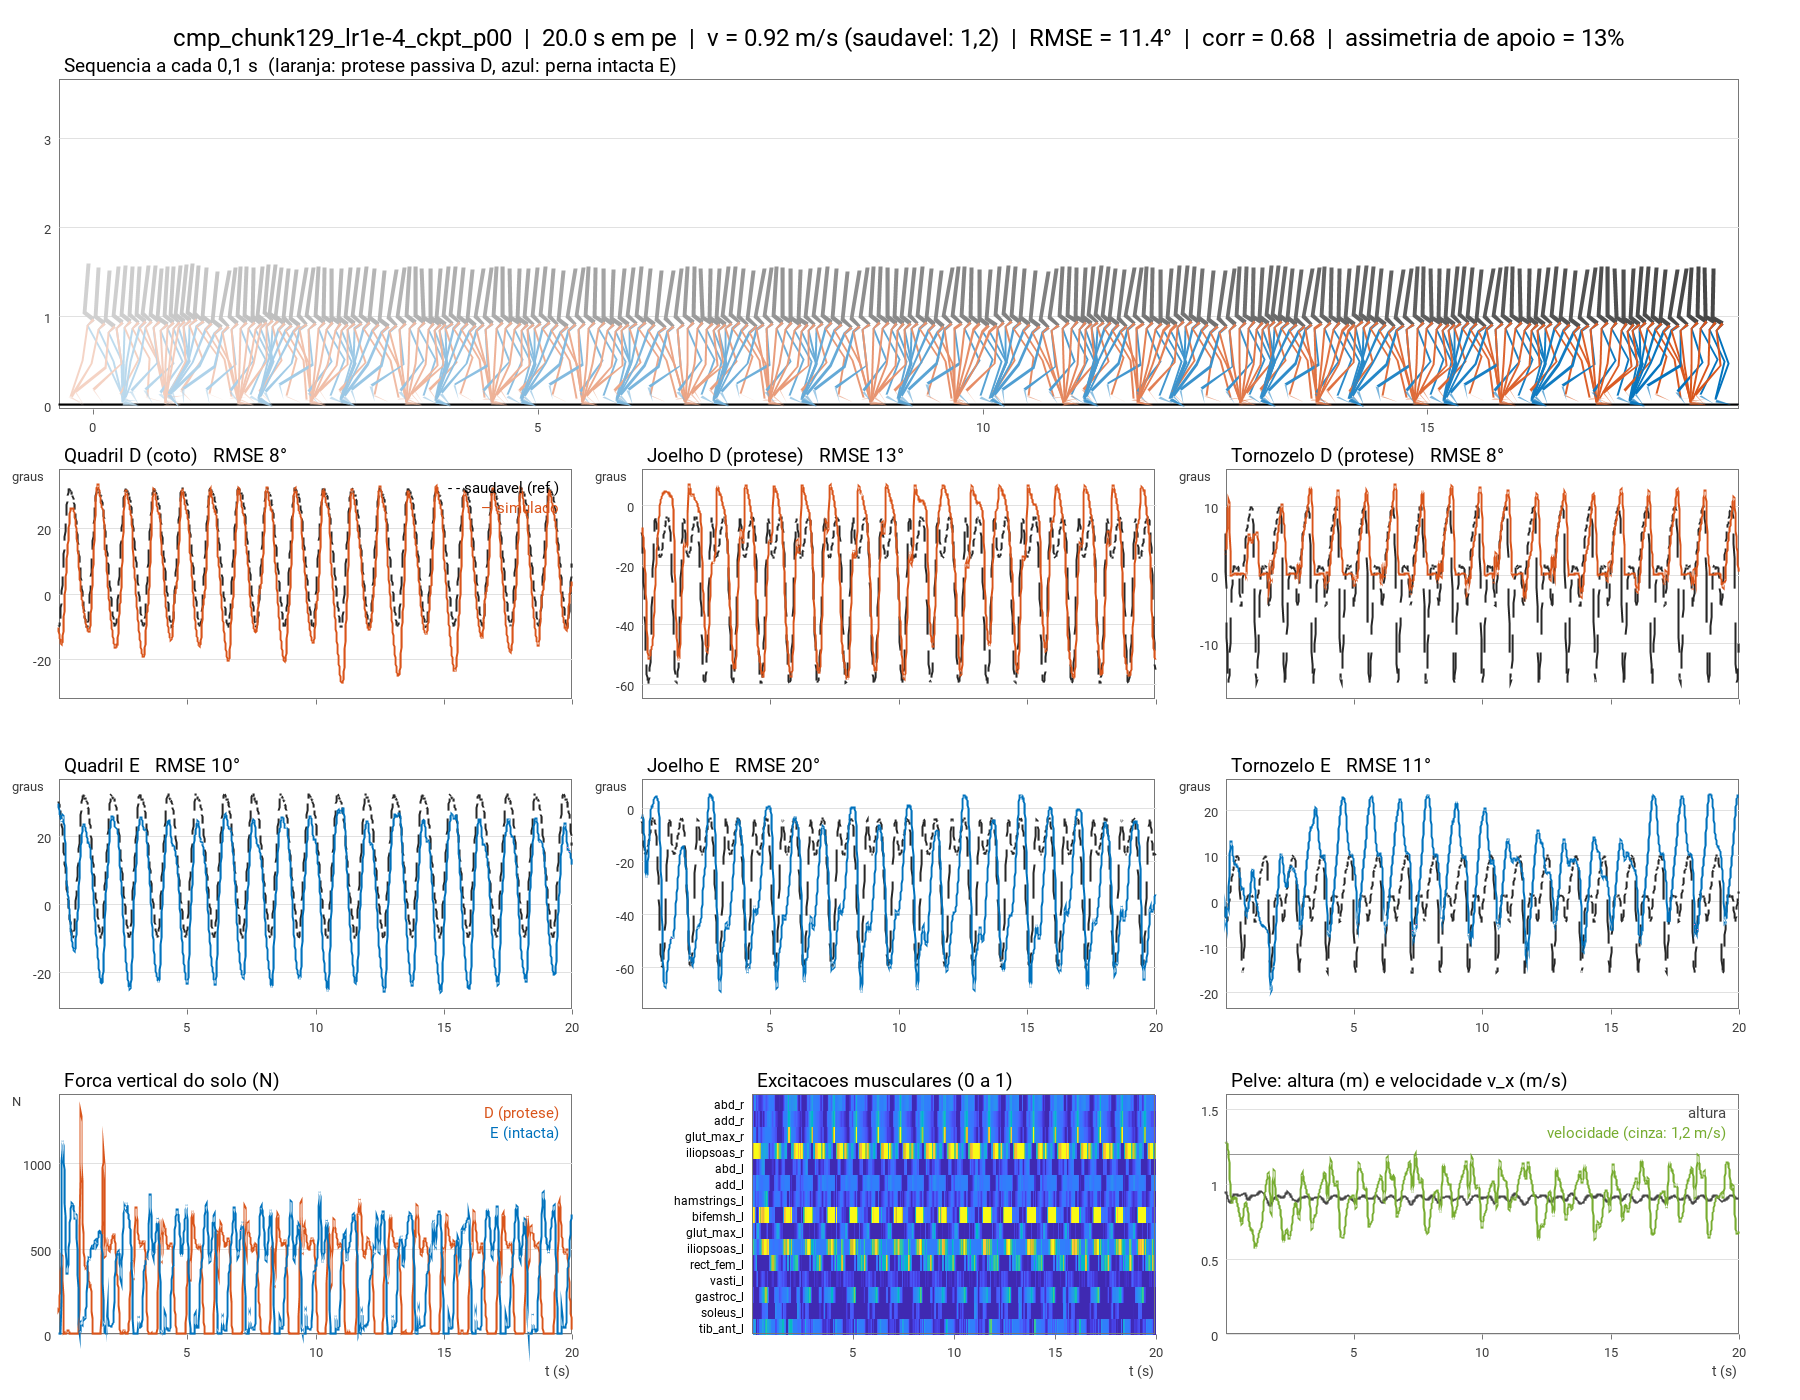
\includegraphics[width=\textwidth]{figs/melhor_agente_resultado.png}
\caption{Melhor agente (bloco 129), 20~s a partir da fase 0. Topo: sequência a cada 0{,}1~s (laranja:
prótese; azul: perna intacta). Meio: ângulos articulares contra a referência saudável (tracejado).
Base: força vertical do solo, excitações musculares e altura e velocidade da pelve.}
\label{fig:result}
\end{figure}

\begin{figure}[H]
\centering
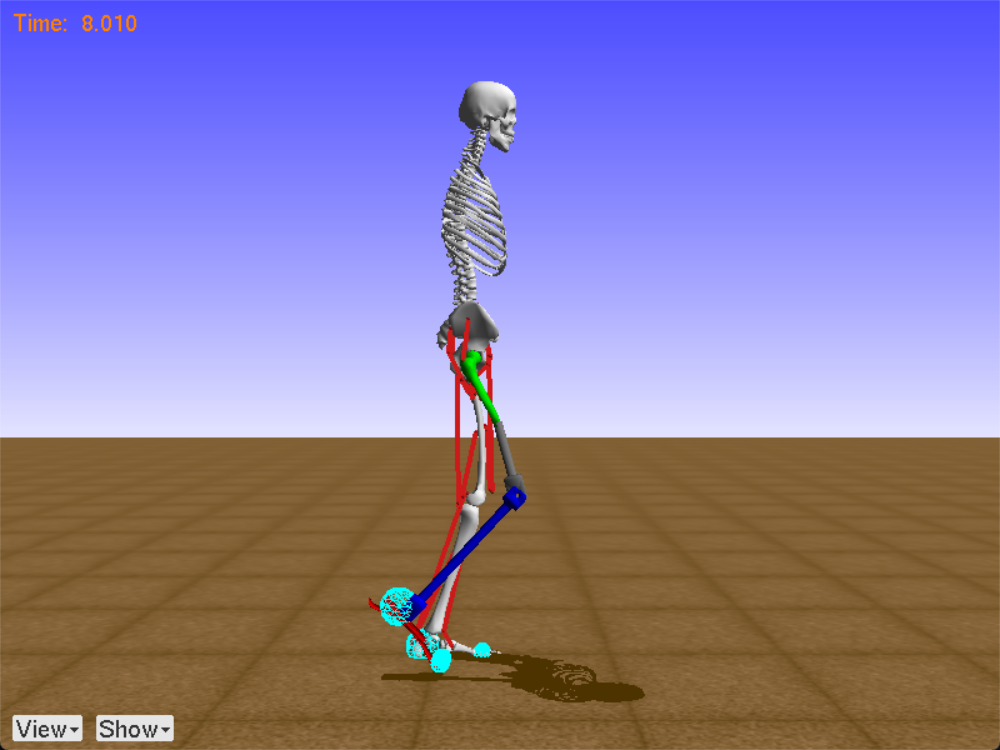
\includegraphics[width=0.24\textwidth]{figs/opensim_t08.png}\hfill
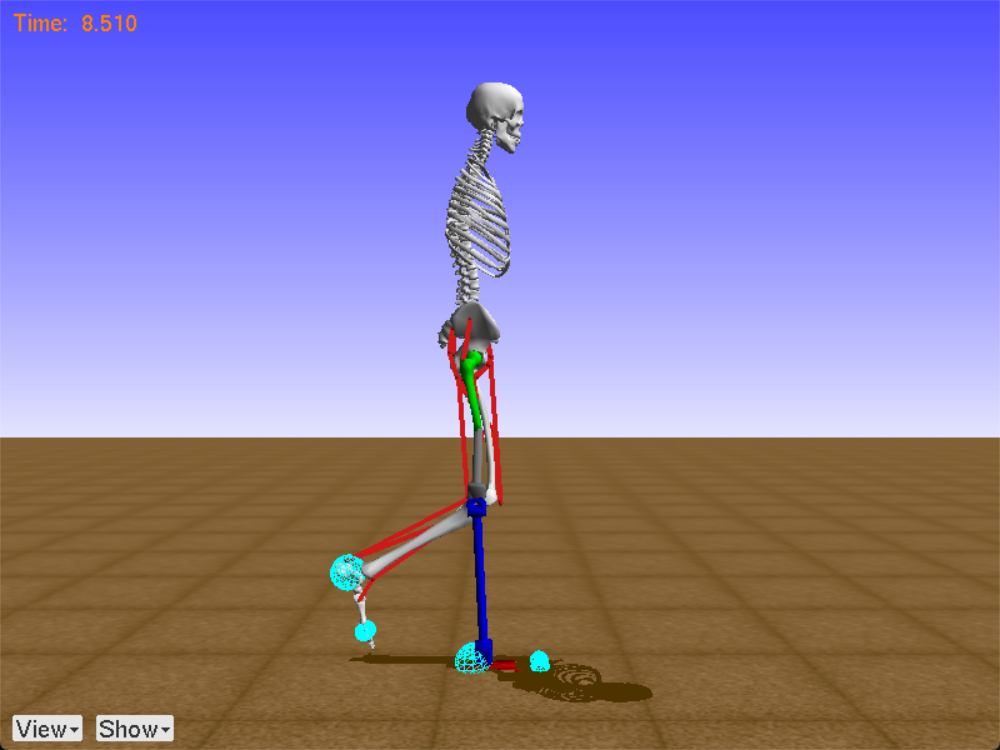
\includegraphics[width=0.24\textwidth]{figs/opensim_t085.png}\hfill
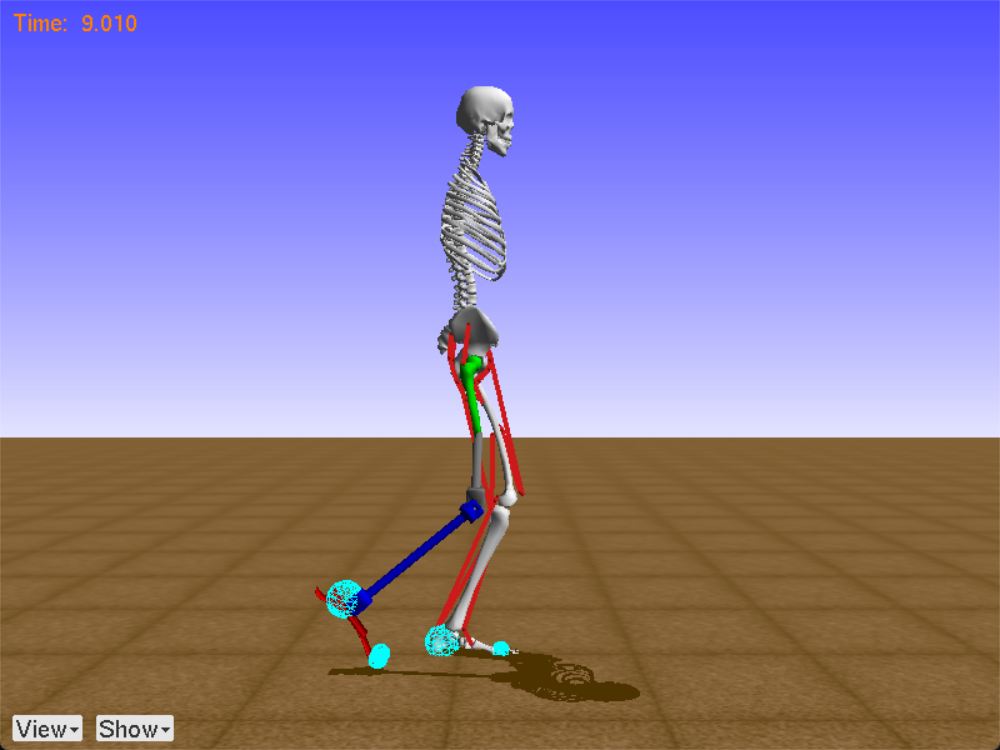
\includegraphics[width=0.24\textwidth]{figs/opensim_t09.png}\hfill
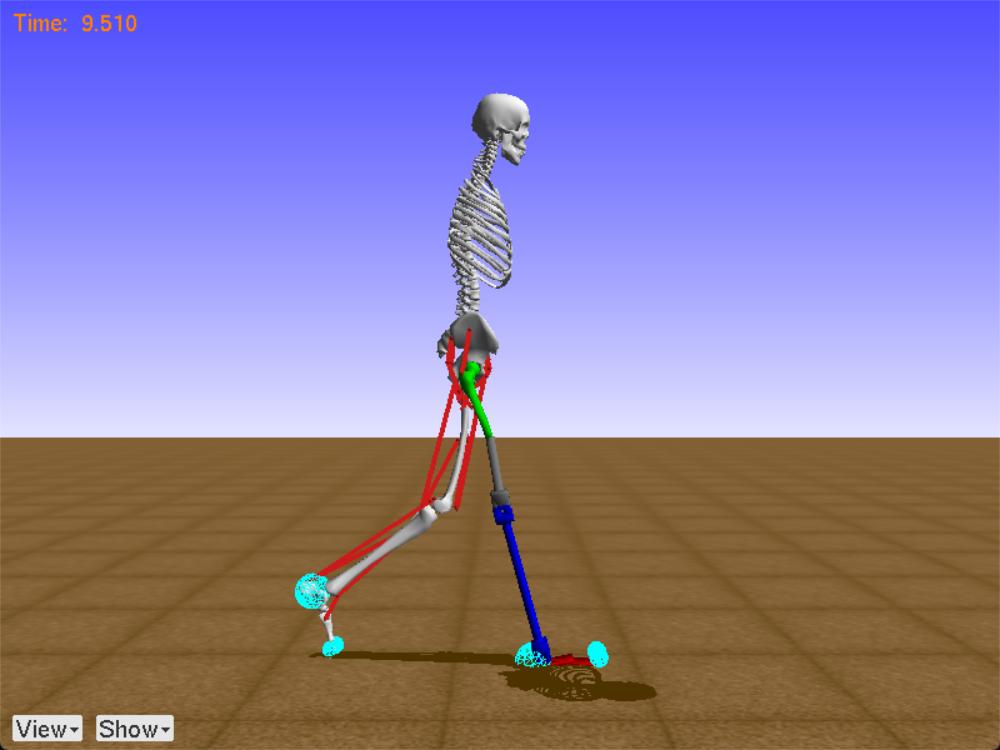
\includegraphics[width=0.24\textwidth]{figs/opensim_t095.png}
\caption{Quadros do visualizador 3D do OpenSim (Simbody) em $t=8{,}0$; $8{,}5$; $9{,}0$ e $9{,}5$~s:
ossos, prótese (encaixe verde, pilão cinza e azul) e músculos (vermelho). Vídeo completo em
\protect\code{results/cmp_chunk129_lr1e-4_ckpt_p00_opensim.mp4}.}
\end{figure}

%=====================================================================
\section{Comparação com a marcha saudável por ciclo}
\label{sec:ciclo}
\subsection{Dados saudáveis e procedimento}
A referência de variabilidade vem do conjunto público de Fukuchi, Fukuchi e Duarte
\cite{fukuchi2018}: 42 adultos saudáveis (24 jovens e 18 idosos), marcha no solo em três velocidades,
com ângulos e cinética já normalizados no ciclo (101 pontos, média por sujeito). Os dados estão no
Figshare sob licença CC BY 4.0. Foram baixados os arquivos em texto (\code{WBDSascii.zip}) e a tabela de
metadados (\code{WBDSinfo.csv}), guardados em \code{data/wbds/}.

\begin{itemize}
  \item \textbf{Velocidade pareada.} O agente anda a 0{,}94~m/s. Por isso a faixa saudável principal
        é a da velocidade \emph{lenta} do dataset, $0{,}86\pm0{,}13$~m/s. A média da velocidade
        \emph{confortável}, $1{,}27\pm0{,}16$~m/s, aparece como linha tracejada.
  \item \textbf{Saudável.} Para cada sujeito, média das pernas direita e esquerda; depois média
        $\pm$1 desvio-padrão entre os 42 sujeitos. Ângulos no plano sagital (flexão de quadril e joelho
        positivas, dorsiflexão positiva). Forças divididas pelo peso corporal (PC).
  \item \textbf{Simulação.} Melhor agente (bloco 129), 4 simulações de 20~s com fases iniciais 0; 0{,}25;
        0{,}5 e 0{,}75 (\code{results/best_p*_traj.mat}). O primeiro segundo é descartado. Cada passada
        vai de um contato inicial (força vertical do pé acima de 20~N) ao seguinte do mesmo pé e é
        normalizada em 101 pontos. Isso dá 65 passadas de cada lado. O sinal do joelho do OpenSim
        (flexão negativa) é invertido, e as forças são divididas pelo peso do modelo (67{,}8~kg).
  \item \textbf{Código.} \code{src/gait_cycle_comparison.m} gera \code{docs/figs/ciclo_comparacao.csv},
        que as Figuras~\ref{fig:ciclo_ang} e~\ref{fig:ciclo_grf} leem diretamente.
\end{itemize}

\pgfplotstableread[col sep=comma]{figs/ciclo_comparacao.csv}\ciclo
\pgfplotstableread[col sep=comma]{figs/ciclo_faixas.csv}\faixas
\begin{figure}[H]
\centering
\begin{tikzpicture}
\begin{groupplot}[group style={group size=2 by 3, horizontal sep=1.6cm, vertical sep=0.9cm,
    xlabels at=edge bottom, xticklabels at=edge bottom},
  width=0.5\textwidth, height=4.6cm, xmin=0, xmax=100, xtick={0,20,...,100},
  grid=major, grid style={black!8}, tick label style={font=\scriptsize}, label style={font=\small},
  title style={font=\small\bfseries}, xlabel={ciclo de marcha (\%)}]
  \nextgroupplot[title={Lado protético (direito)}, ylabel={flexão do quadril ($^\circ$)}] \cyclepanel{hip}{R}{cOrange}
  \nextgroupplot[title={Lado intacto (esquerdo)}] \cyclepanel{hip}{L}{cBlue}
  \nextgroupplot[ylabel={flexão do joelho ($^\circ$)}] \cyclepanel{knee}{R}{cOrange}
  \nextgroupplot \cyclepanel{knee}{L}{cBlue}
  \nextgroupplot[ylabel={dorsiflexão ($^\circ$)}] \cyclepanel{ankle}{R}{cOrange}
  \nextgroupplot \cyclepanel{ankle}{L}{cBlue}
\end{groupplot}
\end{tikzpicture}\\[2pt]
\cyclelegend
\caption{Ângulos articulares sagitais por ciclo de marcha (0~\% = contato inicial do pé do mesmo lado).
Faixa cinza: marcha saudável lenta, média $\pm$1~DP, 42 sujeitos \cite{fukuchi2018}. Tracejado: média
saudável em velocidade confortável. Cores: média $\pm$1~DP das 65 passadas simuladas de cada lado. No lado
protético, o joelho e o tornozelo são as juntas passivas da prótese.}
\label{fig:ciclo_ang}
\end{figure}

\begin{figure}[H]
\centering
\begin{tikzpicture}
\begin{groupplot}[group style={group size=2 by 2, horizontal sep=1.6cm, vertical sep=0.9cm,
    xlabels at=edge bottom, xticklabels at=edge bottom},
  width=0.5\textwidth, height=4.6cm, xmin=0, xmax=100, xtick={0,20,...,100},
  grid=major, grid style={black!8}, tick label style={font=\scriptsize}, label style={font=\small},
  title style={font=\small\bfseries}, xlabel={ciclo de marcha (\%)}]
  \nextgroupplot[title={Lado protético (direito)}, ylabel={vertical (PC)}] \cyclepanel{grfv}{R}{cOrange}
  \nextgroupplot[title={Lado intacto (esquerdo)}] \cyclepanel{grfv}{L}{cBlue}
  \nextgroupplot[ylabel={ântero-posterior (PC)}] \cyclepanel{grfap}{R}{cOrange}
  \nextgroupplot \cyclepanel{grfap}{L}{cBlue}
\end{groupplot}
\end{tikzpicture}\\[2pt]
\cyclelegend
\caption{Forças de reação do solo por ciclo de marcha, em múltiplos do peso corporal (PC). Força
ântero-posterior positiva = propulsão (para a frente). Mesma legenda da Figura~\ref{fig:ciclo_ang}.}
\label{fig:ciclo_grf}
\end{figure}

\subsection{Resultados}
\begin{table}[H]
\centering\small
\caption{Simulação contra a média saudável lenta (\protect\code{docs/figs/ciclo_resumo.csv}). ``Dentro da faixa'' é a
fração do ciclo em que a média simulada fica a até 1~DP da média saudável.}
\begin{tabular}{@{}lrrrrrr@{}}
\toprule
 & \multicolumn{3}{c}{Lado protético} & \multicolumn{3}{c}{Lado intacto} \\
\cmidrule(lr){2-4}\cmidrule(l){5-7}
Variável & RMSE & $r$ & dentro da faixa & RMSE & $r$ & dentro da faixa \\ \midrule
Quadril (flexão) & $9{,}1^\circ$ & 0{,}97 & 49\,\% & $21{,}9^\circ$ & 0{,}13 & 34\,\% \\
Joelho (flexão) & $10{,}1^\circ$ & 0{,}85 & 35\,\% & $36{,}2^\circ$ & $-0{,}70$ & 6\,\% \\
Tornozelo (dorsiflexão) & $4{,}4^\circ$ & 0{,}71 & 48\,\% & $8{,}4^\circ$ & 0{,}43 & 24\,\% \\
GRF vertical & 0{,}14~PC & 0{,}96 & 16\,\% & 0{,}48~PC & 0{,}26 & 3\,\% \\
GRF ântero-posterior & 0{,}08~PC & 0{,}19 & 11\,\% & 0{,}07~PC & 0{,}62 & 24\,\% \\ \midrule
Duração do apoio & \multicolumn{3}{c}{$70{,}3\pm7{,}3$\,\% do ciclo} & \multicolumn{3}{c}{$88{,}2\pm6{,}4$\,\% do ciclo} \\
\bottomrule
\end{tabular}
\end{table}
Nos saudáveis, o apoio dura $64{,}3\pm1{,}5$\,\% do ciclo na velocidade lenta e $62{,}4\pm1{,}2$\,\% na
confortável.

\paragraph{Lado protético.} A forma geral segue a da marcha saudável.
\begin{itemize}
  \item \textbf{Quadril do coto} ($r=0{,}97$): mesmo formato, mas a extensão máxima é maior e chega
        antes, $\approx-16^\circ$ perto de 50\,\% do ciclo, contra $\approx-6^\circ$ perto de 56\,\% no saudável.
  \item \textbf{Joelho protético} ($r=0{,}85$): fica quase estendido durante o apoio, encostando no batente
        perto de 20\,\%. No balanço dobra até $\approx50^\circ$, abaixo dos $\approx60^\circ$ saudáveis, e o pico vem
        mais tarde.
  \item \textbf{Tornozelo protético} ($r=0{,}71$): acompanha a dorsiflexão do apoio, mas não faz a flexão
        plantar do pré-balanço e fica perto de $0^\circ$ no balanço, como esperado de um pé passivo rígido
        ($k=350$~N\,m/rad).
  \item \textbf{Força vertical} ($r=0{,}96$): tem os dois picos. O descarregamento é lento e o apoio se
        estende até $\approx70$\,\% do ciclo.
  \item \textbf{Força ântero-posterior} ($r=0{,}19$): tem um pico positivo atípico perto de 15\,\% e uma
        fase de propulsão menor perto de 50\,\%, com $\approx0{,}08$ contra $\approx0{,}15$~PC. A prótese passiva gera
        pouco impulso no fim do apoio.
\end{itemize}

\paragraph{Lado intacto.} É onde a marcha mais se afasta da saudável. O pé esquerdo fica no ar só
$\approx$0{,}16~s por passada e volta a tocar o solo cedo, com pouca carga (35--150~N), ainda com o joelho
dobrado $\approx$55$^\circ$. Só depois recebe o peso do corpo. Por isso o apoio da perna intacta dura 88\,\%
do ciclo, e o ciclo, que começa nesse toque leve, fica desalinhado da referência: o joelho começa
flexionado, o que dá correlação negativa. Na prática, a perna intacta compensa a prótese: fica mais
tempo no chão e sustenta o corpo, um padrão comum em amputados transfemorais, mas aqui exagerado.

\paragraph{Diferença em relação à assimetria da Tabela~\ref{tab:criterios}.} A assimetria de apoio de 11\,\% calculada
por \code{evaluate_policy} usa limiar de 50~N e conta tempo total de contato; os toques leves de 20--50~N do
pé intacto ficam de fora. Com o limiar de 20~N e a definição por passada desta seção, a diferença de
apoio entre os lados é bem maior (70 contra 88\,\% do ciclo).

\section{Visualização}
%=====================================================================
Nesta máquina, os gráficos do MATLAB travam tanto no modo \code{-batch} quanto ao abrir o desktop por linha
de comando. Por isso a visualização foi feita de dois modos que não dependem deles:
\begin{itemize}
  \item \code{make_media.m}: usa o OpenSim para a cinemática direta (posição de quadris, joelhos,
        tornozelos e esferas de contato a cada amostra) e desenha a figura-resumo e o vídeo de boneco
        diretamente em pixels com \code{insertShape} e \code{insertText}. Grava \code{<tag>_resultado.png},
        \code{<tag>_marcha.mp4} e \code{<tag>_pontos.csv}.
  \item \code{render_opensim.m} + \code{capture_window.ps1}: reproduz a trajetória no visualizador 3D do
        OpenSim (Simbody), com a câmera seguindo a pelve. Cada quadro é capturado da janela por um script
        PowerShell, que mantém a janela sempre por cima. Quadros cobertos por outra janela (céu não azul)
        são capturados de novo. O resultado é \code{<tag>_opensim.mp4}.
  \item Os arquivos \code{<tag>_motion.mot} podem ser abertos no OpenSim GUI (\emph{File $\to$ Load Motion}).
\end{itemize}

%=====================================================================
\section{Desempenho computacional}
%=====================================================================
\begin{itemize}
  \item Bloco de 40 episódios: $\approx$430~s com episódios de 3~s e 600--900~s com episódios de 6~s
        (4 workers, CPU de 12 núcleos lógicos).
  \item O aprendiz roda no processo principal e é o gargalo. Com uma atualização por passo, um bloco levava
        $\approx$920~s; com uma a cada 4 passos, caiu para 150--250~s (episódios de 3~s).
  \item \textbf{GPU:} \code{bench_gpu.m} mediu o custo do aprendiz sem a simulação, usando um ambiente
        falso com as mesmas dimensões. O resultado foi 177~ms por atualização na CPU e 188~ms numa RTX 2060.
        Com redes de 256 neurônios e lote de 256, o tempo vai no custo fixo de cada chamada, não no cálculo.
        A opção \code{'device','gpu'} existe em \code{train_sac}, mas não traz ganho. A simulação
        (OpenSim + \code{ode23}) roda só na CPU.
\end{itemize}

%=====================================================================
\section{Problemas encontrados e soluções}
%=====================================================================
\begin{longtable}{@{}p{6.3cm}p{9.2cm}@{}}
\toprule
Problema & Solução \\ \midrule \endhead
JVM \code{EXCEPTION_ACCESS_VIOLATION} em \code{Coordinate.getValue} & O \code{State} devolvido pelo \code{Manager} era liberado junto com ele. Copiar o estado e, depois, eliminar o \code{Manager}. \\
``State Cache entry out of date'' & Chamar \code{realizeDynamics} após \code{setY}. \\
\code{getStateVariableDerivativeValues} indisponível & Usar \code{getY}/\code{getYDot} do Simbody. \\
Thelen2003 sem \code{ignore_tendon_compliance} & Opção removida. \\
Recompensa negativa incentivava cair & Forma multiplicativa $\text{tarefa}\cdot e^{-P}$ (sempre $\ge0$ enquanto vivo). \\
Termo de velocidade sem gradiente parado & Núcleo mais largo ($k_s$ de 5 para 1{,}5) e mais peso; depois, com a marcha estável, $k_s=2{,}5$ e $w_s=0{,}45$. \\
Aprendiz como gargalo (922~s por bloco) & \code{LearningFrequency = 4}. \\
\code{equilibrateMuscles} falhava em algumas fases & Sortear outra fase (até 6 vezes) e tratar estado inválido como queda. \\
Execução com currículo de assistência degenerou & Reinício sem assistência. \\
Horizonte de 3~s saturado (avaliações paradas em 3--5~s) & Episódios de 6~s e mais peso na velocidade. \\
Política oscilando entre blocos & Taxa de aprendizado de $3\cdot10^{-4}$ para $10^{-4}$, retomando do melhor agente. \\
Gráficos do MATLAB travam em \code{-batch} & Desenho direto em pixels (\code{make_media}) e captura do visualizador Simbody (\code{render_opensim}). \\
\code{setWindowTitle} inexistente na API MATLAB do visualizador & Chamada removida. \\
Janela sobreposta durante a gravação & Janela \code{HWND_TOPMOST} e verificação de cada quadro. \\
\bottomrule
\end{longtable}

%=====================================================================
\section{Limitações e próximos passos}
%=====================================================================
\begin{itemize}
  \item \textbf{RMSE e correlação} ainda fora da meta, principalmente pelos joelhos. O joelho protético
        é uma mola e um amortecedor lineares. Um modelo com freio de apoio ou atrito dependente da carga
        representaria melhor joelhos passivos comerciais e deixaria o apoio mais estável.
  \item \textbf{Velocidade} de 0{,}94~m/s, ainda abaixo dos 1{,}2~m/s da referência. Amputados
        transfemorais costumam andar mais devagar, então talvez a referência deva ser ajustada para essa
        população.
  \item \textbf{Marcha planar}: o próximo estágio é liberar as coordenadas 3D (\code{gaitConfig('planar', false)}).
  \item \textbf{Referência aproximada}: curvas reconstruídas de pontos-chave, não de dados medidos de um
        sujeito.
  \item \textbf{Buffer não persistente}: cada reinício do treino perde o replay buffer, e os primeiros
        blocos pioram.
\end{itemize}

%=====================================================================
\section{Guia de uso}
%=====================================================================
\begin{lstlisting}[numbers=none]
cd src
% treino (retoma de results/sac_checkpoint.mat se existir)
train_sac('nChunks', 150, 'episodesPerChunk', 40, 'workers', 4, 'resume', true, 'lr', 1e-4)
% avaliacao de um agente
S = load('../results/best_agent.mat');
M = evaluate_policy(S.agent, 'assist', 0, 'duration', 20, 'initPhase', 0, 'tag', 'final')
% comparacao robusta de todos os agentes salvos
T = compare_agents('duration', 20, 'phases', [0 .25 .5 .75], 'workers', 6)
% figura-resumo e video de boneco; video no visualizador 3D do OpenSim
make_media('final')
render_opensim('final')
\end{lstlisting}

\begin{thebibliography}{9}
\bibitem{fukuchi2018} C.~A. Fukuchi, R.~K. Fukuchi e M.~Duarte. A public dataset of overground and
treadmill walking kinematics and kinetics in healthy individuals. \emph{PeerJ}, 6:e4640, 2018.
\url{https://doi.org/10.7717/peerj.4640}. Dados: \url{https://doi.org/10.6084/m9.figshare.5722711} (CC BY 4.0).
\end{thebibliography}

\appendix
%=====================================================================
\section{Referência dos arquivos}
%=====================================================================
\begin{longtable}{@{}p{4.2cm}p{11.3cm}@{}}
\toprule
Arquivo & Função \\ \midrule \endhead
\code{src/gaitConfig.m} & Todos os parâmetros: modelo, integrador, músculos, coordenadas, ganhos, prótese, assistência, término e recompensa. Também calcula $F_{\max}$ e a máscara músculo $\times$ junta. \\
\code{src/healthyGaitReference.m} & Curvas periódicas de marcha saudável (quadril, joelho, tornozelo, adução). \\
\code{src/ProstheticGaitEnv.m} & Ambiente de RL: monta o modelo (prótese passiva, assistência, controlador), \code{reset} com RSI, \code{step} com integração \code{ode23}, controlador-base, observação, recompensa e gravação da trajetória. \\
\code{src/train_sac.m} & Cria ou retoma o agente SAC, treina em blocos em paralelo, avalia, salva checkpoints e histórico. \\
\code{src/evaluate_policy.m} & Simulação determinística, métricas, \code{.mot}, \code{_traj.mat} e \code{_traj.csv}. \\
\code{src/compare_agents.m} & Avaliação robusta de vários agentes em várias fases iniciais. \\
\code{src/gait_cycle_comparison.m} & Segmenta as passadas simuladas, normaliza no ciclo e compara com a marcha saudável do dataset público (média $\pm$1~DP). \\
\code{data/wbds/} & Dataset público de marcha saudável \cite{fukuchi2018} (arquivos em texto processados em \code{proc/}). \\
\code{src/make_media.m} & Figura-resumo e vídeo de boneco desenhados em pixels. \\
\code{src/render_opensim.m} & Vídeo no visualizador 3D do OpenSim. \\
\code{src/capture_window.ps1} & Captura da janela do visualizador (PowerShell, user32/GDI). \\
\code{src/bench_gpu.m} & Custo do aprendiz SAC em CPU e GPU. \\
\code{src/test_deriv.m} & Tempo de avaliação de $\dot{\mathbf y}$ e comparação de integradores. \\
\code{src/test_baseline.m}, \code{src/sweep.m} & Testes do controlador-base com ação zero e varredura de parâmetros. \\
\code{results/} & Checkpoints, agentes salvos, \code{train_log.csv}, \code{train_console.log}, avaliações, figuras e vídeos. \\
\bottomrule
\end{longtable}

%=====================================================================
\section{Código-fonte}
%=====================================================================
\subsection{\texorpdfstring{\protect\code{gaitConfig.m}}{gaitConfig.m}}
\lstinputlisting{codigo/gaitConfig.m}
\subsection{\texorpdfstring{\protect\code{healthyGaitReference.m}}{healthyGaitReference.m}}
\lstinputlisting{codigo/healthyGaitReference.m}
\subsection{\texorpdfstring{\protect\code{ProstheticGaitEnv.m}}{ProstheticGaitEnv.m}}
\lstinputlisting{codigo/ProstheticGaitEnv.m}
\subsection{\texorpdfstring{\protect\code{train_sac.m}}{train_sac.m}}
\lstinputlisting{codigo/train_sac.m}
\subsection{\texorpdfstring{\protect\code{evaluate_policy.m}}{evaluate_policy.m}}
\lstinputlisting{codigo/evaluate_policy.m}
\subsection{\texorpdfstring{\protect\code{compare_agents.m}}{compare_agents.m}}
\lstinputlisting{codigo/compare_agents.m}
\subsection{\texorpdfstring{\protect\code{gait_cycle_comparison.m}}{gait_cycle_comparison.m}}
\lstinputlisting{codigo/gait_cycle_comparison.m}
\subsection{\texorpdfstring{\protect\code{make_media.m}}{make_media.m}}
\lstinputlisting{codigo/make_media.m}
\subsection{\texorpdfstring{\protect\code{render_opensim.m}}{render_opensim.m}}
\lstinputlisting{codigo/render_opensim.m}
\subsection{\texorpdfstring{\protect\code{capture_window.ps1}}{capture_window.ps1}}
\lstinputlisting[language={}, morecomment={[l]\#}]{codigo/capture_window.ps1}
\subsection{\texorpdfstring{\protect\code{bench_gpu.m}}{bench_gpu.m}}
\lstinputlisting{codigo/bench_gpu.m}
\subsection{\texorpdfstring{\protect\code{test_deriv.m}}{test_deriv.m}}
\lstinputlisting{codigo/test_deriv.m}
\subsection{\texorpdfstring{\protect\code{test_baseline.m}}{test_baseline.m}}
\lstinputlisting{codigo/test_baseline.m}
\subsection{\texorpdfstring{\protect\code{sweep.m}}{sweep.m}}
\lstinputlisting{codigo/sweep.m}

\end{document}
